The full physical information about a process is contained in a complete set of \textit{helicity amplitudes}.

They are calculated by selecting all external states of particles to be the states with definite helicity \todo{define what helicity is}.

It is well known that helicity amplitudes exhibit nice physical properties such as trivialization of gauge-invariance and
manifestation of Poincare symmetry \todo{some references}.

From a technical perspective this means that helicity amplitudes are ``good'' objects to compute. \todo{this is very rough formulation}

As we mentioned before, amplitudes with loops exhibit divergences, which forces us
to use dimensional regularization.\footnote{other regularization methods exist \todo{reference}, but this is out of the scope of this thesis}


Formally then the corresponding space is infinite-dimensional \todo{reference Collins}, and
it can be made to ``coincide'' with the finite-dimensional one whenever $D$ takes integer values.

In CDR we replace $SO(1,3)$ invariance by $SO(1,D-1)$.
In HV by $SO(1,3)\otimes SO(D-4)$.

After all divergences are cancelled, the limit $D\to4$ is taken and the physical results are recovered.

All particle transform as irreducible representations of Poincare group in $D$ dimensions,
so the number of states becomes infinite.
This raises the question as to how to define a helicity amplitude in the framework of dimensional regularization.


\section{Tensor Decomposition and Projectors}

In this section we review a way to define helicity amplitudes in dimensional regularization through
$D$-dimensional projectors.

This approach has been used in a number of computations \cite{Garland:2002ak, Moch:2002hm, Glover:2003cm, Glover:2004si,Gehrmann:2009vu,Gehrmann:2011aa}.
It's relation to HV scheme and helicity amplitudes has been recently further clarified \cite{Peraro:2019cjj}.

One starts with decomposing an amplitude with unspecified external states into all possible $D$-dimensional tensor structures compatible
with symmetries. One finds a basis of these structures and finds corresponding $D$-dimensional projectors.
At this point the calculation is done in CDR using $D$-dimensional tensor and Clifford algebras.

Then one switches to the HV scheme by decomposing projectors in $4$ and $(D-4)$ parts,
and chooses four-dimensional helicity states as a basis.
And helicity amplitudes are found by constructing appropriate linear combinations of projectors.
Some of the initial coefficients become irrelevant.

The complexity and number of initial projectors grows very fast with the number of external particles, as was demonstrated in \cite{Peraro:2019cjj}.

Projection approach is a backwards way of doing helicity amplitudes.

Note that asking for helicity amplitudes makes sense only in HV scheme.


\section{HV Helicity Amplitudes from Embedding of States}

We show how to obtain helicity amplitudes directly, without complicated projectors,
for vector and spinor particles.
We achieve this by working in HV scheme from the get-go, and by
choosing an appropriate embedding of the physical four-dimensional state in $D$ dimensions.

This is trivially achieved for gluon helicity states: these
are vector particles and any four-dimensional polarization state
can be embedded in a generic $D$-dimensional space by filling 
the remaining components of the vector with zeros. 
For fermion states, however, the embedding is less trivial as 
the nature of the $D$-dimensional Clifford algebra means that
there is no single associated state in $D$-dimensions.  

As such, one might wonder if it is possible at all to unambiguously 
define four-dimensional helicity amplitudes with external
fermions. In this section we describe how we
address this problem, inspired by the approach of
refs.~\cite{Glover:2003cm,Glover:2004si}.
 
This generalizes the prescription of EGKM for one-loop to multi-loop and
multi-quark (also massive).

\subsection{Embedding of Vector States}

\subsection{Embedding of Spinor States}
\label{sec:Clifford}


There are several consistent regularization schemes that can be
chosen, see
e.g.~ref.~\cite{Gnendiger:2017pys} for a recent review, and our
discussion applies to both the conventional
dimensional regularization (CDR) and the 't Hooft-Veltman (HV)
schemes. The two schemes differ in the way
vector particles (gluons in our case) are treated,
and we follow 
the description given in the reference
above.\footnote{Except for the meaning of $D_s$, which we use 
to denote the dimension of the CDR and HV singular vector 
fields, to differentiate it from the dimensional regulator $D$.}
In CDR, all vector fields are vectors in a space of dimension
$D_s=4-2\epsilon$. In
HV, one distinguishes between \emph{regular} and 
\emph{singular} vector 
fields. The former do not lead to any singularities and 
are considered to be
strictly four-dimensional objects. The
latter are a source of singularities and are 
$D_s$-dimensional vectors. For our purposes, this means
that gluons whose momentum we integrate over are 
$D_s$ dimensional, and external gluons whose momentum
we do not integrate over are
four dimensional. The two schemes are consistent,
in that their contributions to NNLO computations can be related by known
transition rules~\cite{Broggio:2015dga}, but as we
shall see below the HV scheme introduces some simplification in
the calculation.


We consider fermions in $D_s$ dimensions, as is for instance
necessary when a CDR gluon or a singular HV gluon is emitted 
from a quark line. If the fermion line closes upon itself, as in
e.g.~the $N_f$ corrections to gluon amplitudes
(i.e., corrections with a closed massless-quark loop), 
we only need the defining
property of the Clifford algebra
\begin{equation} \label{eqn:defClifford}
\{ \gamma_{[D_s]}^\mu, \gamma_{[D_s]}^\nu \} = 
2 g_{[D_s]}^{\mu\nu}\mathbb{1}_{[D_s]}^{\vphantom{\mu\nu}} \,,
\end{equation}
where we explicitly write the dimension $D_s$
as a subscript of the $\gamma$-matrices and the metric, and
use a metric with mostly-minus Minkowski signature, 
$g_{[D_s]}=\mathrm{diag}\{1, -1 , ... , -1 \}$.
Here $\mathbb{1}_{[D_s]}$ is the identity operator in the representation space of 
the Clifford algebra.
In the presence of external fermions, however, 
we must also describe the corresponding states and
an explicit
representation of the $D_s$-dimensional Clifford algebra is
required. Since we are ultimately interested in specifying
four-dimensional
external states, it is furthermore convenient to construct 
the representation in a factorized way starting from four dimensions
(see e.g.~refs.~\cite{Kreuzer:susylectures,Collins:1984xc}).
We thus consider a Clifford algebra
in $D_s$ dimensions as the tensor product of a
four-dimensional and a $(D_s-4)$-dimensional one:
\begin{equation}\label{eqn:cliffordrecursion}
%
(\gamma_{[D_s]}^\mu)_{a\kappa}^{\,b\lambda}  = \left\{ 
\begin{array}{ll} 
		\left(\gamma_{[4]}^\mu\right)_a^{\;b} \,
		\delta_\kappa^\lambda\,, &\quad  0\le\mu \le 3 \,,\\&\\
		\left(\tilde\gamma_{[4]}\right)_a^{\;b} 
		\left(\gamma_{[D_s-4]}^{(\mu-4)}\right)_\kappa^{\;\lambda}\,, 
        &\quad \mu > 3 \,,
\end{array}
		\right.
%
\end{equation}
where $\tilde\gamma_{[4]}\equiv i(\gamma_{[4]}^0
\gamma_{[4]}^1 \gamma_{[4]}^2 \gamma_{[4]}^3)$, such that 
$(\tilde\gamma_{[4]})^2 =\mathbb{1}_{[4]}$ is the identity
operator
in the four-dimensional algebra.
The indices $a,b$ denote the spinor indices in the
four-dimensional algebra and $\kappa,\lambda$ the ones of the 
$(D_s-4)$-dimensional one.
The $\gamma^\mu_{[D_s-4]}$ form themselves a 
$(D_s-4)$-dimensional Clifford algebra with signature
$g_{[D_s-4]}=\mathrm{diag}\{ -1 , ... , -1 \}$.
In amplitude calculations we naturally encounter products of
$\gamma$ matrices, and in this paper we will mainly focus
on chains of $\gamma_{[D_s-4]}$ matrices. 
We thus define a convenient basis for these chains, 
constructed by anti-symmetrizing over their Lorentz
indices and given by (see e.g.~\cite{Kreuzer:susylectures})
\begin{align}\label{eq:basisGammaChainDs}
\gamma_{[D_s-4]}^{\mu_1 \ldots \mu_n} = \frac{1}{n!} \sum_{ \sigma\in S_n} \sgn(\sigma) \gamma_{[D_s-4]}^{\mu_{\sigma(1)}} \ldots \gamma_{[D_s-4]}^{\mu_{\sigma(n)}}\,,
\end{align}
where $S_n$ denotes the set of all permutations of $n$
integers and $\sgn(\sigma)$ the signature of the permutation
$\sigma\in S_n$.

The spinor states associated with the $D_s$-dimensional 
Clifford algebra live in a $D_t$-dimensional space.\footnote{We 
remind the reader that although $D_t=2^{D_s/2}$ for any 
finite-dimensional representation, $D_t$ is set to $4$ in 
dimensional regularization \cite{Collins:1984xc}.}
For four-dimensional momenta they can be constructed from a 
tensor-product representation as
%%
\begin{equation} 
\label{eq:fermionicStates}
\psi_{s,a \kappa} =  (u_h)_a (\eta^i)_\kappa \,,
\quad\mbox{and}\quad
\bar \psi_s^{a \kappa} = 
(\bar u_h)^{a}  (\bar \eta_i)^\kappa\,,
\end{equation}
%
where we have introduced an index $s=\{h, i \}$ to denote the
polarization states in terms of spinors of the four- and 
$(D_s-4)$-dimensional subspaces. 
Without loss of generality we can
require that $(\eta^i)_\kappa$ and $(\bar \eta_i)^\kappa$ 
be dual to each other,
%
\begin{equation}
\label{eqn:qspinors}
(\bar \eta_i)^\kappa (\eta^j)_\kappa = \delta_i^j\,,
\end{equation}
and choose a canonical basis for the 
spinors in the $(D_s-4)$-dimensional space,
i.e.~set $(\eta^i)_\kappa=\delta^i_\kappa$.
%
In an on-shell computation in $D_s$ dimensions we use the 
spinor states defined in eq.~\eqref{eq:fermionicStates}
as external fermion wave functions.
Given the choice of a canonical basis for the 
$(D_s-4)$-dimensional states, we can identify the
$(D_s-4)$ polarization label $i$ with the spinor index 
$\kappa$ in eq.~\eqref{eq:fermionicStates}.
Thus, in the following we only insert four-dimensional spinors
and keep track of the $(D_s-4)$-dimensional embedding with 
the open $(D_s-4)$ spinor index.
We note that a bilinear of external $(D_s-4)$-dimensional
spinors $\eta \bar \eta'$ can  be expressed in terms of the 
basis of $\gamma$-matrix chains introduced in 
eq.~\eqref{eq:basisGammaChainDs},
%
\begin{equation}\label{eq:etaetaP}
\eta \bar \eta' = \mathbb{1}_{[D_s-4]} f +  
\gamma_{[D_s-4]}^{\nu_1} f_{\nu_1} + 
\gamma_{[D_s-4]}^{\nu_1\nu_2} f_{\nu_1\nu_2} + \ldots \,,
\end{equation}
%
where the $\{ f , f_{\nu_1}, f_{\nu_1\nu_2},\cdots \}$ are the
constant coefficients in the decomposition.
In loop calculations, this naively introduces reference vectors and tensors that can yield linear
dependence on the components of the loop-momenta beyond four
dimensions, see e.g.~\cite{Badger:2017gta,Anger:2018ove},
in contrast with
what happens, for instance, in the case of amplitudes with
only gluons.
We only mention this here as an observation since, as we 
shall see in the remaining of this paper, this will not be an
issue with our definition of helicity amplitudes.

The tensor product representation of the Clifford algebra is
particularly useful to separate four- and 
$(D_s-4)$-dimensional spinor indices in $\gamma$-matrix chains. 
Indeed, a product of
$\gamma$ matrices where some
Lorentz indices are within four dimensions (denoted
$\mu_i$),
and some are beyond four dimensions (denoted $\hat\mu_i$) is
split into two blocks, a four-dimensional and a 
$(D_s-4)$-dimensional one. For instance, we have
\begin{align}
  \begin{split}
    \left(\gamma_{[D_s]}^{\mu_1}
    \gamma_{[D_s]}^{\hat \mu_2}
    \gamma_{[D_s]}^{\mu_3}
    \gamma_{[D_s]}^{\hat\mu_4}\right)_{a\kappa}^{\,b\lambda} &=
    -\left(
    \gamma_{[D_s]}^{\mu_1}
    \gamma_{[D_s]}^{\mu_3}
    \gamma_{[D_s]}^{\hat \mu_2}
    \gamma_{[D_s]}^{\hat\mu_4} \right)_{a\kappa}^{\,b\lambda} \\
    &=-\left( 
    \gamma_{[4]}^{\mu_1}
    \gamma_{[4]}^{\mu_3}
    \right)_a^{\,b}   \,\left(
    \gamma_{[D_s-4]}^{(\hat \mu_2-4)}
    \gamma_{[D_s-4]}^{(\hat \mu_4-4)}
    \right)_\kappa^{\,\lambda}  \,.
  \end{split}
\end{align}
Consider now contracting the above
product of $\gamma$ matrices with a four-dimensional fermion state,
such as the $u$ and $\bar u$ spinors:
\begin{equation}
	\label{eq:tensorChain}
	\bar u^a
	\left(\gamma_{[D_s]}^{\mu_1}
	\gamma_{[D_s]}^{\hat \mu_2}
	\gamma_{[D_s]}^{\mu_3}
	\gamma_{[D_s]}^{\hat\mu_4}\right)_{a\kappa}^{\,b\lambda}
	u_b=
	-\left(\bar u
	\gamma_{[4]}^{\mu_1}
	\gamma_{[4]}^{\mu_3}
	u\right)
	\left(
	\gamma_{[D_s-4]}^{(\hat \mu_2-4)}
	\gamma_{[D_s-4]}^{(\hat \mu_4-4)}
	\right)_\kappa^{\,\lambda}\,.
\end{equation}
The result is a tensor with open indices in the
$(D_s-4)$-dimensional space.
We recall that these are in one-to-one
correspondence with a $(D_s-4)$-dimensional state, and the above expression (\ref{eq:tensorChain}) is
thus equivalent to a contraction with on-shell helicity states in $D_s$ dimensions.
%
Our ultimate goal is the calculation of amplitudes relevant for 
cross-section computations, and we must then understand which
tensor structures beyond four dimensions are necessary. 
This will be done in the next subsections.

We finish this section with two comments. First, we note that in the
HV scheme this tensor decomposition results in simpler expressions
than in CDR. Consider for instance the tree-level $q\bar q\to Q\bar
Q$ amplitude
\begin{equation}
  \left(M^{(0)}\right)_{\kappa_1 \kappa_2}^{\lambda_1 \lambda_2}
  \;\sim\;\; 
  \bar u^{a_1}
  \left(
  \gamma_{[D_s]}^\mu
  \right)_{a_1 \kappa_1}^{b_1 \lambda_1}
  u_{b_1}
  \,\,
  \bar u^{a_2}
  \left(
  \gamma_{[D_s]\mu}
  \right)_{a_2 \kappa_2}^{b_2 \lambda_2}
  u_{b_2}
  \,.
\end{equation}
In the HV scheme, the gluon between the two quark lines is
four dimensional, i.e., $\mu\leq3$, while
in the CDR scheme, the gluon is $D_s$ dimensional.
From eq.~\eqref{eqn:cliffordrecursion} we thus get
\begin{equation}
  \label{eq:HVvsCDR}
  \left(M^{(0)}\right)_{\kappa_1,\kappa_2}^{\lambda_1,\lambda_2}
  =
  \begin{cases}
    M^{(0)}_{0}\, \delta_{\kappa_1}^{\lambda_1}
    \delta_{\kappa_2}^{\lambda_2}& \textrm{in HV,}\\
    M^{(0)}_{0}\, \delta_{\kappa_1}^{\lambda_1}
    \delta_{\kappa_2}^{\lambda_2}+
    M^{(0)}_{1}\,\Bigl(\gamma_{[D_s-4]}^{\mu}\Bigl)_{\kappa_1}^
    {\lambda_1}
    \Bigl(\gamma_{[D_s-4]\mu}\Bigl)_{\kappa_2}^{\lambda_2}
    &\textrm{in CDR,}
  \end{cases}
\end{equation}
where the $M_i^{(0)}$ are coefficients that are determined from
products of four-dimensional $\gamma$-matrices contracted with
four-dimensional spinors.
In the HV scheme the amplitude is
determined by a single coefficient, 
while in CDR two are needed. In the
remainder of this paper we thus choose to work in the HV scheme.
Nevertheless, our discussion
generalizes to the CDR scheme in a straightforward way.

The second comment we wish to make is that, 
although in this section we consider $D_s=4-2\epsilon$, which
means the Clifford algebra defined in 
eq.~\eqref{eqn:cliffordrecursion} is infinite dimensional, in
numerical calculations one might need to construct an explicit
representation of the Clifford algebra and thus
take $D_s$ to be an even integer (larger than 4).
The construction 
of eq.~\eqref{eqn:cliffordrecursion} still holds and, in fact, 
it can be iterated: any even $D_s$ can be reached
by constructing a tensor product of the
$(D_s-2)$ algebra with a 2-dimensional algebra, even if the 
$(D_s-2)$ algebra 
was already constructed as a tensor product of two
algebras.

\subsection{Tensor Decomposition in $D_s-4$}
\label{sec:HelAmplHV}

We consider a helicity amplitude $M$, expanded in 
perturbation theory, with the $k$-th order term written as
$M^{(k)}$.
We saw previously that these are tensors in the
$(D_s-4)$-dimensional spinor space, see
eq.~\eqref{eq:HVvsCDR} for an explicit example.
Here we introduce a basis for the associated tensor space in the
spinor indices beyond four dimensions, whose elements are 
denoted as $v_n$. In general,
the basis depends on the physical process described 
by $M$ and on the order $k$ in the perturbative
expansion. We will suppress this dependence for simplicity of 
the notation and write
\begin{equation}
  M^{(k)}= \sum_n  v_n M^{(k)}_n,
\label{eq:tensorDecomposition}
\end{equation}
where the $M^{(k)}_n$ are computed from
$\gamma_{[4]}^{\mu}$ matrices and external states in four dimensions, and the tensor structure
of the amplitude in the spinor indices beyond four dimensions is
fully contained in the $v_n$.
In the following, we explicitly construct the basis $\{v_n\}$
for two families of amplitudes: those with a pair $q\bar q$ of
external
quarks and any number of external gluons, and
those with two pairs $q\bar q$ and $Q\bar Q$
of external quarks (of either different or identical
flavor) and any number of external gluons.

The different tensors $v_n$ are constructed by contracting the
Lorentz indices of chains of $\gamma_{[D_s]}$ matrices with
other Lorentz vectors in the amplitude after all loop
integrations have been performed. The remaining objects that
carry Lorentz indices are four-dimensional external momenta,
four-dimensional polarization vectors and chains of $\gamma_{[D_s]}$
matrices. Any Lorentz index in a $\gamma_{[D_s]}$-matrix 
chain that is contracted with a four-dimensional object becomes
four-dimensional, contributing only a trivial tensor structure 
in the $(D_s-4)$-dimensional space. For instance, if $\varepsilon_\mu$ represents a
four-dimensional polarization vector of an external gluon,
\begin{equation}
	\label{eq:trivialTens1}
	\varepsilon_\mu
	\left(
	\gamma_{[D_s]}^\mu
	\right)_{a\kappa}^{b\lambda}
	=\varepsilon_\mu\left(\gamma_{[4]}^\mu
	\right)_{a}^{b}\delta_{\kappa}^{\lambda}\,.
\end{equation}
Similarly when two Lorentz indices are contracted inside the 
same chain of $\gamma_{[D_s]}$ matrices, the tensor structure
beyond four dimensions is trivial, as follows from:
\begin{equation}
	\label{eq:trivialTens2}
	\left(\gamma_{[D_s]}^\mu\right)_{a \kappa}^{b_1 \lambda_1}
        \left(\gamma_{[D_s]\mu}^{\phantom{\mu}}\right)_{b_1 \lambda_1}^{b \lambda}
	=D_s\delta_{a}^{b}\delta_{\kappa}^{\lambda}\,.
\end{equation}
Non-trivial tensors $v_n$ are obtained by contracting
Lorentz indices of two chains of $\gamma_{[D_s-4]}$ matrices.
The basis introduced in eq.~\eqref{eq:basisGammaChainDs} 
for these chains is particularly useful for
computing these contractions.

Let us consider an amplitude with a pair $q\bar q$ of external
quarks and any number of external gluons. There is a single
chain of $\gamma_{[D_s-4]}$ matrices and,
as there are no other objects with $(D_s-4)$ indices, it
follows from the discussion above that
for this case there is a single term in the sum of
eq.~\eqref{eq:tensorDecomposition}:
\begin{equation}\label{eq:decompqqbar}
	M^{(k)}
	(q,\bar q,g,\ldots,g)
	=w_0\,M^{(k)}_0\,,\qquad
	\textrm{with}\quad
	(w_0)_{\kappa}^{\lambda}=\delta_{\kappa}^{\lambda}\,.
\end{equation}
We define the dual tensor
$w^0$ such that $w_0\cdot w^0=1$, with more details given in
appendix~\ref{sec:identities}.

Let us now consider an amplitude with two quark pairs of 
different flavors, $q\bar q$ and $Q\bar Q$, and any number of
gluons. We can now contract Lorentz indices between two 
different chains of $\gamma$ matrices, and the basis 
$\{v_n\}$ is then larger in this case. Using the basis for the
$\gamma$-matrix chains introduced in 
eq.~\eqref{eq:basisGammaChainDs}, we construct the associated
basis $\{v_n\}$:
\begin{align}
  \begin{split} \label{eqn:4qtensors}
    (v_0)_{\kappa_1\kappa_2}^{\lambda_1\lambda_2}   = &
    \delta_{\kappa_1}^{\lambda_1} \delta_{\kappa_2}^{\lambda_2}\,, \\
    (v_1)_{\kappa_1\kappa_2}^{\lambda_1\lambda_2}=
    &(\gamma_{[D_s-4]}^{\mu_1} )_{\kappa_1}^{\lambda_1} 
    (\gamma_{[D_s-4]\mu_1}^{\phantom{\mu}})_{\kappa_2}^{\lambda_2}\,, \\
    & \vdots\\
    (v_m)_{\kappa_1\kappa_2}^{\lambda_1\lambda_2}=
    &(\gamma_{[D_s-4]}^{\mu_1 \ldots  \mu_m})_{\kappa_1}^{\lambda_1}
    (\gamma_{[D_s-4]\mu_1 \ldots \mu_m}^{\phantom{\mu}})_{\kappa_2}^{\lambda_2}\,,\\
    & \vdots\,
  \end{split}
\end{align}
where we have made explicit the indices in the $
(D_s-4)$-dimensional space.
The basis $\{v_n\}$ is infinite dimensional for
$D_s=4-2\epsilon$ (because there are infinitely many independent
terms of the form of eq.~\eqref{eq:basisGammaChainDs}), but at
each order in the perturbative
expansion only a finite number of basis elements contribute, 
as follows from inspecting the corresponding Feynman diagrams.
We thus have
\begin{equation} \label{eqn:4qampltensor}
	M^{(k)} (q,\bar q,Q,\bar Q,g,\ldots,g) =\sum_{n=0}^{n_k} v_n M^{(k)}_n\,.
\end{equation}
In the HV scheme, the decomposition is independent of the number
of external gluons. In particular,
the value of $n_k$ can be determined from the amplitude with no 
external gluons, by examining the Feynman diagrams
with the most singular gluons. 
These are ladder-type four-point diagrams with the 
gluons in the rungs. We find for instance that $n_0=0$,
$n_1=3$ and $n_2=5$ for tree-level, one- and two-loop
amplitudes, respectively. Our decomposition is similar to the 
one presented in ref.~\cite{Glover:2004si}, but differs in the
choice of basis tensors in eq.~\eqref{eq:tensorDecomposition}.

In practical calculations, one is interested in computing
specific coefficients $M^{(k)}_n$ in the decomposition
of eq.~\eqref{eq:tensorDecomposition}. We construct the
basis $\{v_n\}$ such that this operation is trivial, i.e., it
satisfies
\begin{equation}\label{eqn:vnproducts}
	v_n^\dagger\cdot v_m=c_n\delta^n_m\,,
	\quad
    c_0(D_s) = 1\,\quad\mbox{and}\quad  c_{n>0}(D_s)={\cal O}(\epsilon)\,.
\end{equation}
The calculation of the coefficients $c_n$ requires some 
technical operations on $\gamma$ matrices that we present in
appendix~\ref{sec:identities}.
We then construct the dual basis $\{v^n\}$, with elements
\begin{equation}\label{eq:dualBasis}
	v^n=\frac{1}{c_n} (v_n)^\dagger\,.
\end{equation}
Using the dual basis, we directly get
\begin{equation}\label{eqn:helampl}
  M^{(k)}_n = v^n \cdot M^{(k)}.
\end{equation}

Finally let us consider an amplitude with two identical quark
pairs, which can be constructed by anti-symmetrizing the
distinct-flavor amplitude $M^{(k)}$ over the two
flavors~\cite{DeFreitas:2004kmi,Glover:2004si}.
It is then easy to see that the decomposition of
eq.~\eqref{eq:tensorDecomposition} requires an enlarged basis
compared to the distinct-quark case of
eq.~\eqref{eqn:4qtensors}. We thus define the tensors
$\{\tilde v_n\}$ as
\begin{equation}\label{eq:basisIdentical}
	(\tilde v_n)_{\kappa_1\kappa_2}^{\lambda_1\lambda_2}=
	(v_n)_{\kappa_1\kappa_2}^{\lambda_2\lambda_1}\,,
\end{equation}
and the decomposition of eq.~\eqref{eq:tensorDecomposition}
is over the sets $\{v_n\}$ and $\{\tilde v_n\}$.
The basis tensors satisfy
\begin{equation}\label{eq:dualBasisIdentical}
	v_nv^m=\delta^m_n\,,\qquad
	\tilde v_n\tilde v^m=\delta^m_n\,,\qquad
	v_n\tilde v^m=
	\delta^m_0\,\delta_{n,0}+\mathcal{O}(\epsilon)\,,
\end{equation}
where the set $\{\tilde v^n\}$ is constructed to be dual to
$\{\tilde v_n\}$ in the same way as in 
eq.~\eqref{eq:dualBasis}.

We finish this subsection with a comment on the case where $D_s$
is a finite integer $D_s^0$. 
All the discussion above holds, but one
must be careful with a small detail. 
The basis of the Clifford algebra in 
eq.~\eqref{eq:basisGammaChainDs} now contains only a finite 
number of terms, and the basis of tensors $\{v_n\}$ is
consequently restricted by the dimension $D^0_s$. 
If one wants to compute the coefficient of a given tensor 
$v_i$, one must thus choose $D_s^0$ large enough such
that $v_i \in \{v_n\}$. Nevertheless, one can check that a 
calculation done in $D_s^0$ dimensions agrees 
with the $D_s=D_s^0$ limit of the same calculation done in
generic $D_s$.


\subsection{Relevant Tensor Coefficients}

We have established that helicity amplitudes in dimensional
regularization are tensors in the $(D_s-4)$-dimensional space and
introduced a basis of that space on which we can decompose the
amplitude.  We should in
principle compute all coefficients in the decomposition. However, it
turns out that in a given phenomenological application not all
coefficients may be relevant. We discuss below the two cases
involving external quarks pertinent to the subject of this 
paper, the amplitudes with only external gluons being trivial in
this regard.

\paragraph{Two-loop $q\bar qg\ldots g$ amplitude:}
For the case of an amplitude with a pair $q\bar q$ of external
quarks and any number of external gluons,
there is a single coefficient to determine, 
see eq.~\eqref{eq:decompqqbar}. At order $k$ in perturbation
theory we call this object $A^{(k)}$. It is
computed using
\begin{equation}\label{eq:qqProj}
    A^{(k)}(q,\bar q,g,\ldots,g)=M^{(k)}_0(q,\bar q,g,\ldots,g) =
	w^0\cdot M^{(k)}(q,\bar q,g,\ldots,g)\,,
\end{equation}
i.e. by
tracing over the $(D_s-4)$-dimensional indices of the
fermion line. In this paper we are mostly interested in $k=2$.

\paragraph{Two-loop $q\bar qQ\bar Qg\ldots g$ amplitude:}
For a
two-loop amplitude with two quark pairs of 
different flavors, $q\bar q$ and $Q\bar Q$, and any number of
gluons there are in principle six coefficients to determine. 
However, in an NNLO computation (that is not loop-induced) 
the two-loop amplitude is 
interfered with the tree amplitude, which has a single tensor
structure in the HV scheme. The contribution we must compute is of the form
\begin{equation}\label{eq:qqQQProj}
  \left(M^{(0)}\right)^\dagger M^{(2)}=
  \left(M^{(0)}_0\right)^\dagger M^{(2)}_0\,,
\end{equation}
where we have used the orthogonality of the tensors
$v_n$ and the fact that $c_0(D_s)=1$, see 
eq.~\eqref{eqn:vnproducts}. 
For NNLO corrections, it is
thus sufficient to compute the coefficients
$M^{(2)}_0$ through
\begin{equation}
  \label{eq:AmplitudeDefinition}
  A^{(2)}(q,\bar q,Q,\bar Q,g,\ldots,g)=
  M^{(2)}_0 = v^0 \cdot 
  M^{(2)}(q,\bar q,Q,\bar Q,g,\ldots,g),
\end{equation}
which amounts to computing the 
$(D_s-4)$-dimensional trace of $M^{(2)}$ on
each fermion line.  
We define the amplitude
$A^{(k)}(q,\bar q,Q,\bar Q,g,\ldots,g)$ for any order $k$
in an analogous way.

This approach is similar to the one of
ref.~\cite{Glover:2004si} and is in
agreement with the prescription of ref.~\cite{Anger:2018ove}.
On a first look, it might however look inconsistent with the 
way $q\bar qQ\bar Q$ helicity amplitudes are defined in
ref.~\cite{DeFreitas:2004kmi}. Written in the formalism
we have introduced in this section, the authors compute
\begin{equation}
	\label{eq:AmpDefAlt}
	\tilde v^0\cdot M^{(2)}
	(q,\bar q,Q,\bar Q)\,,
\end{equation}
and, given the relations of eq.~\eqref{eq:dualBasisIdentical}, this
would not necessarily give the same 
$A^{(2)}(q,\bar q,Q,\bar Q)$ defined in 
eq.~\eqref{eq:AmplitudeDefinition}. For
phenomenological applications, however, 
one can show that only the
so-called \emph{finite remainder} is relevant 
\cite{Weinzierl:2011uz},
and we now show that the choices of 
eqs.~\eqref{eq:AmplitudeDefinition} and \eqref{eq:AmpDefAlt}
give the same result for this quantity.\footnote{This was 
already pointed out by the authors of 
ref.~\cite{DeFreitas:2004kmi}, who discuss the agreement of 
their finite remainder results with those of ref.~\cite{Glover:2004si}.}
We first recall that the infrared poles of a renormalized QCD
amplitude $M_R$ have a universal structure, and we can
write an amplitude in terms of its universal pole structure
and a finite remainder
which we will denote $\CF$
\cite{Catani:1998bh,Sterman:2002qn,Becher:2009cu,Gardi:2009qi}.
More explicitly, 
for a two-loop amplitude we have
\begin{equation}\label{eq:remainderDef}
	M^{(2)}_R=
	\mathbf{I}^{(2)}M^{(0)}_R
	+\mathbf{I}^{(1)}M^{(1)}_R
	+\CF^{(2)}\,,
\end{equation}
where $\mathbf{I}^{(1)}$ and $\mathbf{I}^{(2)}$ are operators in color
space. We refer the reader to appendix~\ref{sec:IR} for 
explicit expressions for these operators in the leading-color
approximation of the amplitudes considered in this paper. Since
$\CF^{(2)}$ is finite, we have
\begin{equation}
	v^0\cdot \CF^{(2)}
	=\tilde v^0\cdot \CF^{(2)}+\mathcal{O}(\epsilon),
        \label{eq:RemainderEquivalence}
\end{equation}
and the remainder computed from 
eq.~\eqref{eq:AmplitudeDefinition} thus agrees with the 
one computed from eq.~\eqref{eq:AmpDefAlt}. 


\subsection{Parametrization of Integrands of Amplitudes with External Fermions}
\label{sec:ParamIntegrands}

Since our representation of fermion amplitudes is manifestly
Lorentz invariant in $(D_s-4)$ dimensions prior to loop
integration, the integrands of fermion amplitudes can be
decomposed in terms of the same set of master integrands and
surface terms as those used for amplitudes with gluons only \cite{Abreu:2017xsl,Abreu:2017hqn}.
We demostrate this below.

 To see this point more
explicitly, consider the
integrand $M_k(\ell_l)$
of an amplitude with an arbitrary
number of quark lines where the subscript $k$ encodes the
dependence on the $(D_s-4)$ spinor 
indices.\footnote{This can be viewed as a generalization of the
decomposition in eq.~\eqref{eq:tensorDecomposition} to the
integrand level.} We can write the integrand in the form
\begin{equation}
  M_k(\ell_l) = \sum_{n,m} f^{\rho_1 \cdots \rho_n, \sigma_1
  \cdots \sigma_m}_{k}
  \left(\prod_{i=1}^n \vec{\mu}_{1 \, \rho_i}\right)
  \left(\prod_{j=1}^m \vec{\mu}_{2 \, \sigma_i}\right),
\end{equation}
with the tensors $f^{\rho_1 \cdots \rho_n, \sigma_1\cdots \sigma_m}_{k}$ implicitly defined. By construction, they
depend on the $(D_s-4)$ components of the loop momenta through
the Lorentz invariant scalar products $\mu_{ij}$. The
$(D_s-4)$ Lorentz indices we write explicitly can only be 
carried in $f^{\rho_1 \cdots \rho_n, \sigma_1\cdots \sigma_m}_{k}$ by $(D_s-4)$-dimensional $\gamma$-matrices or
metric tensors.
In our definition \eqref{eq:tensorDecomposition} of helicity 
amplitudes, the $(D_s-4)$-dimensional spinor indices are to be
contracted with invariant tensors, leading to traces of
$\gamma_{[D_s-4]}$ matrices which
can be expressed in terms of metric tensors. Consequently, the
Lorentz indices in a contraction of $f^{\rho_1 \cdots \rho_n, \sigma_1\cdots \sigma_m}_{k}$ with an invariant tensor
are carried by metric tensors only.
Hence, after contraction with invariant tensors, 
the integrand only depends on $\mu_{ij}$.

In contrast, evaluating amplitudes that introduce a reference
axis in the $(D_s-4)$-dimensional space
would lead in general to a dependence on the components of the
$\vec\mu_i$ and thus on the $r_i$ terms. 
This is the case for instance when considering
gluon-polarization components in the $(D_s-4)$ dimensions 
(as required in the CDR scheme) or generic values of the 
$(D_s-4)$-dimensional spinors $\eta_i$, as written explicitly in eq.~\eqref{eq:etaetaP}. 
The latter has been reported in \cite{Fazio:2014xea,Badger:2017gta}.



\subsection{Identical Quarks}
Finally, we now show that in the case of two pairs of
identical quarks we can also use the
definition of eq.~\eqref{eq:AmplitudeDefinition} 
for NNLO phenomenology.
The relevant contribution is the interference of the 
tree-level amplitude with the remainder, i.e.
\begin{equation}
  \left(M^{(0)} - \tilde{M}^{(0)}\right) \cdot \left( \CF^{(2)} - \tilde{\CF}^{(2)}\right)
  =
  \left(M^{(0)}_0 - \tilde{M}^{(0)}_0 \right) \left( v_0\cdot \CF^{(2)} - \tilde{v}_0\cdot \tilde{\CF}^{(2)}\right) + O(\eps),
  \label{eq:LikeInterference}
\end{equation}
where we denote with tildes the flavor exchanged objects.  Here, we
have used the orthogonality of the $v_n$ and $\tilde{v}_n$ up to
$O(\eps)$ to simplify the expression. Importantly, the right hand side
of eq.~\eqref{eq:LikeInterference} now only contains terms that can be
computed through the definition of 
eq.~\eqref{eq:AmplitudeDefinition}.


When considering amplitudes with two identical quark lines, contributions where
index contractions lead to a single trace as in figure~\ref{fig_SingleTrace} 
should also be considered. Nevertheless, at the level of the
finite remainder, amplitudes with identical quarks can be obtained by
antisymmetrizing distinct-flavor
expressions~\cite{DeFreitas:2004kmi,Abreu:2018jgq} obtained from
eq.~\eqref{eq:defAmpsTensb}. Thus, our results are sufficient for 
NNLO QCD phenomenological studies of processes involving 
identical quarks.

%%%%%%%%%%%%% FIGURE %%%%%%%%%%%%%%%%%%
\begin{figure}[]
  \begin{center}
    \begin{tikzpicture}[scale=.9]
    % 5 point masters
    \node at (0,0){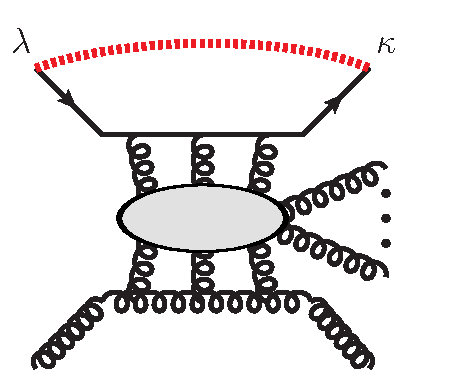
\includegraphics[scale=0.5]
    {figures/singleQuark.pdf}};
    % 5 point masters
    \node at (7,-.1){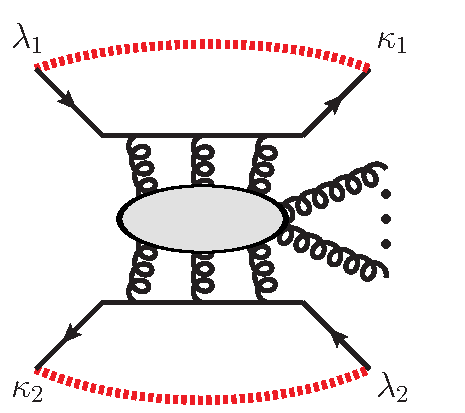
\includegraphics[scale=0.5]
    {figures/doubleTrace.pdf}};
\end{tikzpicture}
\end{center} 
\caption{Contraction of the open $(D_s-4)$-dimensional spinor indices for amplitudes
with external quarks: each quark line closes upon itself.
Indices connected by red dashed lines are traced over.}
\label{fig_traces}
\end{figure}
%%%%%%%%%%%%% FIGURE %%%%%%%%%%%%%%%%%%
\begin{figure}[]
  \begin{center}
  	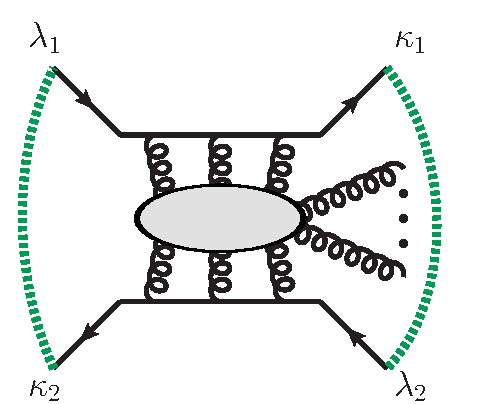
\includegraphics[scale=0.5]
    {figures/singleTrace.pdf}
\end{center} 
\caption{Alternative contraction of $(D_s-4)$-dimensional spinor indices leading to a
single trace. Indices connected by green dashed lines are traced
over.}
\label{fig_SingleTrace}
\end{figure}





\subsection{Chiral couplings ($\gamma_5$)}

\todo{do I really want this to be here\ldots?}
At least general remarks should be written I think that inconsistent algebras cannot
be applied here due to non-analyticity. So the only consistent method should be when $\gamma_5$ commutes
with higher dim. matrices.

\section{$D_s$-Dependence From Dimensional Reduction}
Here we explain how to improve the extraction of $D_s$-dependence.
This is crucial for amplitudes with external fermions due to the exponential scaling of the representation.


The amplitudes $A$ defined in eq.~\eqref{eq:defAmpsTens} are polynomials in $D_s$,
\begin{equation}
  A(D_s) = \sum_{i=0}^{N} \mathcal{K}_i~D_s^{i}\ ,
  \label{eq:ds-poly}
\end{equation}
where $N$, the maximal power of $D_s$, 
varies depending on the process, the loop order, and the choice of tensor structure 
in eq.~\eqref{eq:tensorDecomposition}.
For the amplitudes considered in this paper $N\leq2$.
In this section we will suppress all arguments of $A$ and only keep track of the 
dependence on~$D_s$.
%
In a numerical framework, $A(D_s)$ can only be evaluated for integer $D_s$ values for which 
the particle states are well defined.
To be able to set $D_s=4-2\epsilon$ in the HV scheme, the knowledge of the coefficients $\mathcal{K}_i$ is required.
One way to obtain them is to reconstruct the polynomial \eqref{eq:ds-poly} from
a sample of $(N+1)$ integer values of $D_s$.
This procedure is known as dimensional reconstruction \cite{Giele:2008ve} and has  previously been applied
in \cite{Ellis:2008ir,Boughezal:2011br,Abreu:2017xsl,Abreu:2017hqn}.

While being generic and straightforward to implement, this approach has drawbacks which
become particularly evident in amplitudes with fermions.
%
The dimension of the spinor representation scales exponentially (as $2^{D_s/2}$) with $D_s$,
as opposed to the linear scaling of the vector representation.
Furthermore, the external spinor states with definite helicity can be embedded consistently
only for even values of $D_s$,
which pushes the sample values higher compared to the case of vector particles in the loops.
Beyond the obvious detrimental effect on the numerical complexity, the dimensionality of the
spinor representation determines the number of terms entering the evaluation of the traces
to obtain the helicity amplitudes through  eq.~\eqref{eq:defAmpsTens}. For
the case of amplitudes with multiple external quark pairs this makes the computation
of traces unnecessarily time consuming.

These considerations motivate the search for more efficient alternatives to dimensional
reconstruction. Here we employ one such alternative, based on the idea of
dimensional reduction, which has recently been presented in ref.~\cite{Anger:2018ove} 
and already applied to the computation of one-loop amplitudes in ref.~\cite{Anger:2017glm}.
In the remainder of this section we give a brief overview of this method 
and refer the reader to ref.~\cite{Anger:2018ove} for more technical details.

We start by rearranging eq.~\eqref{eq:ds-poly} in the following way:
\begin{equation}
  A(D_s) = \sum_{i=0}^{N} \tilde{\mathcal{K}}_i~(D_s-D_0)^{i},
  \label{eq:ds-poly-alt}
\end{equation}
where $D_0$ is some \textit{base} dimension, and the coefficients $\tilde{\mathcal{K}}_i$
can be obtained by a linear transformation of the coefficients $\mathcal{K}_i$ in eq.~\eqref{eq:ds-poly}.
It turns out that, given a suitable choice of $D_0$,
the dependence of $A(D_s)$ on degrees of freedom higher than $D_0$ can
be captured in a kinematic-independent way.  
This observation allows one to analytically separate this
dependence, and thus evaluate each coefficient $\tilde{\mathcal{K}}_i$
directly. Furthermore, these evaluations are then performed in the base
dimension $D_0$, resulting in spinor representations of much lower dimensionality
compared to those encountered in the framework of dimensional reconstruction.

For reasons that will become clear shortly, one chooses the base
dimension $D_0$ to be the minimal dimension which allows to embed 
all loop-momentum components without introducing new relations.
For two-loop amplitudes we have $D_0=6$, and we
shall specialize to this case henceforth. We write the metric tensor as
a direct sum,
  \begin{align}
    \label{eq:ds-split-metric}
    g^{\mu\nu}_{[D_s]}  = g^{\mu\nu}_{[D_s-6]} + g^{\mu\nu}_{[6]},  \qquad
    g^{\mu\nu}_{[D_s-6]}g^{\phantom{\mu\nu}}_{\mu\nu\,[6]} = 0\,,
  \end{align}
  and the gamma matrices as a direct product 
  (see e.g.~\cite{Collins:1984xc,Kreuzer:susylectures}),
\begin{equation}
  (\gamma_{[D_s]}^\mu)_{a\kappa}^{\,b\lambda}  = \left\{ 
    \begin{array}{ll} 
      \left(\gamma_{[6]}^\mu\right)_a^{\;b} \,
      \delta_\kappa^\lambda\,, &\quad  0\le\mu \le 5 \,,\\&\\
      \left(\gamma^\star_{[6]}\right)_a^{\;b} 
      \left(\gamma_{[D_s-6]}^{(\mu-6)}\right)_\kappa^{\;\lambda}\,, 
      &\quad \mu \geq 6 \,,
    \end{array}
    \right.
    \label{eq:ds-gamma}
\end{equation}
where $\gamma^\star_{[6]}$ is a six-dimensional analogue of $\gamma_5$ in four dimensions, i.e.
$\{\gamma^\star_{[6]},\gamma_{[6]}^\mu\} = 0$ for all $\mu \in \{0,5\}$, and $(\gamma^\star_{[6]})^2 = 1$.
The product representation allows us to factorize any chain of gamma matrices into a product of $6$- and $D_s-6$-dimensional gamma-matrix chains.
Then, using the fact that the trace of a direct product of two matrices is the product of their traces,
we can split the traces required to obtain the coefficients of tensor structures in eq.~\eqref{eq:tensorDecomposition}
as follows:
\begin{equation}
  \Tr\left(\prod_{\mu_i\in \mathcal{G}}\gamma^{\mu_i}_{[D_s]}\right) =
  \Tr\left(\prod_{\mu_i\in \tilde{\mathcal{G}}}\gamma^{\mu_i}_{[D_s-6]}\right) \cdot
  \Tr\left(\prod_{\mu_i\in \mathcal{G}}\gamma^{\mathfrak{I}(\mu_i)}_{[6]}\right),
  \label{eq:ds-split-traces}
\end{equation}
where the product on the left-hand side is over a sequence $\mathcal{G}$ of $D_s$-dimensional Lorentz indices,
$\tilde{\mathcal{G}} = \{ \mu_i \in \mathcal{G} ~\vert~ \mu_i \geq 6 \}$, and the map $\mathfrak{I}$ is defined as
\begin{equation}
  \mathfrak{I} : \mu \to
    \begin{cases}
      \mu, & 0\le\mu \le 5\,, \\
      \star, & \mu \geq 6\,.
    \end{cases}
\end{equation}
The traces of $\prod_{\mu_i\in\tilde{\mathcal{G}}}\gamma^{\mu_i}_{[D_s-6]}$ can be 
evaluated analytically using well-known Clifford algebra identities,
which produce sums of products of $g^{\mu_i\mu_j}_{[D_s-6]}$.
%
The crucial observation is that the only object to be contracted with the indices beyond 
$(D_s-6)$ is $g^{\mu\nu}_{[D_s-6]}$.
This is ensured by our choice of the base dimension.
These indices then always contribute terms of the form $g^\mu_{[D_s-6]\mu} = (D_s-6)$, 
generating contributions to the coefficients $\tilde{\mathcal{K}}_i$ with $i>0$ 
in eq.~\eqref{eq:ds-poly-alt}. At this point, all degrees of freedom beyond $(D_s-6)$
are traded for polynomials in $(D_s-6)$ with integer factors, and the coefficients
$\tilde{\mathcal{K}}_i$ are expressed in terms of six-dimensional objects only.

\todo{Put examples of tree and 1-loop.}

\subsection{Dimensionally Reduced Feynman Rules}
\label{sec:DsFeynRules}
In the table~\ref{tab:Ds-FeynRules} we list the color-ordered Feynman rules for vertices involving the scalar particles introduced in section~\ref{sec:Ds}.
The $(D_s-6)$-dimensional part of these rules can be fully contracted in each Feynman diagram yielding kinematic-independent factors.
\begin{table}[h]
  \centering
  \begin{minipage}[t]{0.4\textwidth}
    \small
  \begin{tabular}{cl}
    $\vcenter{\hbox{\hspace{-2ex}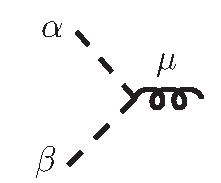
\includegraphics[width=13ex]{figures/Vssg}}}$ & $ \frac{i}{\sqrt{2}}(p_2-p_1)^\mu~ g^{\alpha\beta}_{[D_s-6]}$ \\
    $\vcenter{\hbox{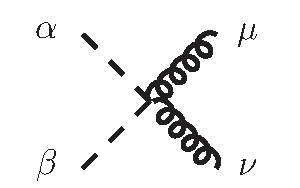
\includegraphics[width=15ex]{figures/Vssgg}}}$ & $ -\frac{i}{2}~g^{\mu\nu}_{[6]}~g^{\alpha\beta}_{[D_s-6]}$ \\
    $\vcenter{\hbox{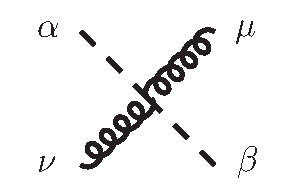
\includegraphics[width=15ex]{figures/Vsgsg}}}$ & $ i~g^{\mu\nu}_{[6]}~g^{\alpha\beta}_{[D_s-6]}$ \\
  \end{tabular}
  \end{minipage}
  \quad
  \begin{minipage}[t]{0.5\textwidth}
    \small
  \begin{tabular}{cl}
    $\vcenter{\hbox{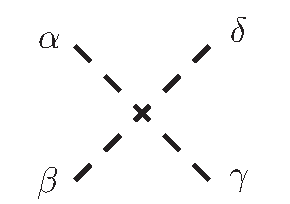
\includegraphics[width=15ex]{figures/Vssss1}}}$ &
      $
      \begin{aligned}
        i~g^{\alpha\gamma}_{[D_s-6]} g^{\beta\delta}_{[D_s-6]} - ~ & \\
                \frac{i}{2}~(g^{\alpha\beta}_{[D_s-6]} g^{\gamma\delta}_{[D_s-6]} & + g^{\alpha\delta}_{[D_s-6]} g^{\beta\gamma}_{[D_s-6]})
      \end{aligned}
      $ \\
        $\vcenter{\hbox{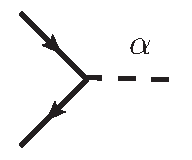
\includegraphics[width=11ex]{figures/VqqsR}}}$ & $- \frac{i}{\sqrt{2}}~\gamma^\star_{[6]} \gamma^\alpha_{[D_s-6]}$ \\
        $\vcenter{\hbox{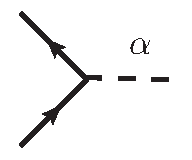
\includegraphics[width=11ex]{figures/VqqsL}}}$ & $ \frac{i}{\sqrt{2}}~\gamma^\star_{[6]} \gamma^\alpha_{[D_s-6]}$ \\
  \end{tabular}
  \end{minipage}
  \caption{Color-ordered Feynman rules for vertices with scalar particles explicitly introduced by dimensional reduction of gluons.}
  \label{tab:Ds-FeynRules}
\end{table}

\FloatBarrier

From a Feynman diagrammatic perspective, the contributions to the
coefficients of the polynomial in $(D_s-6)$
can be represented by introducing a scalar particle. 
The Feynman rules associated to this particle can be readily
derived from dimensional reduction of the original Feynman rules of the
theory \cite{Bern:2002zk,Badger:2013gxa,Giele:2008ve,Anger:2018ove} by
applying the relations \eqref{eq:ds-split-metric} and \eqref{eq:ds-gamma}.
We list them in the appendix \ref{sec:DsFeynRules} for convenience.
To illustrate this procedure we now give an example. 
Consider a decomposition of a Feynman diagram with $D_s$-dimensional particles on the 
left-hand side of figure~\ref{fig:ds-example-diagram}. The four non-vanishing 
contributions after evaluating partial traces and contracting all 
$(D_s-6)$-dimensional indices are shown on the right-hand side, 
where the scalars are introduced to represent what remains of these contractions.

\begin{figure}
  \newlength\diagramWidth
  \setlength{\diagramWidth}{18ex}
  \centering
  \begin{align*}
    \vcenter{\hbox{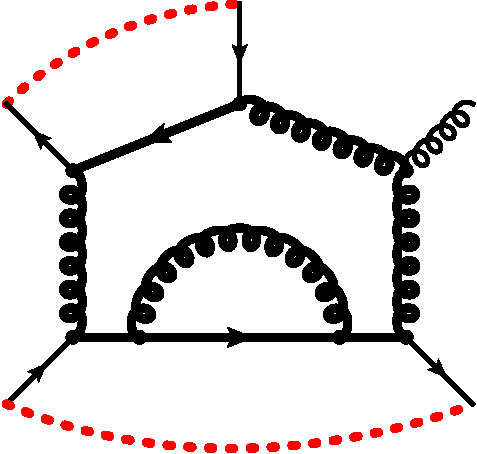
\includegraphics[width=\diagramWidth]{figures/Ds-example_B.pdf}}} \hspace{-10ex} & \hspace{15ex} = \hspace{6ex}
    \vcenter{\hbox{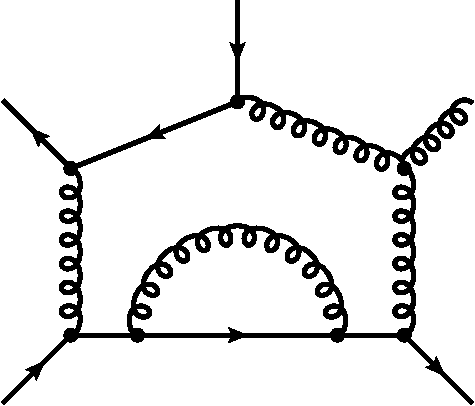
\includegraphics[width=\diagramWidth]{figures/Ds-example.pdf}}} \quad +\\
    \Big(~ &
    \vcenter{\hbox{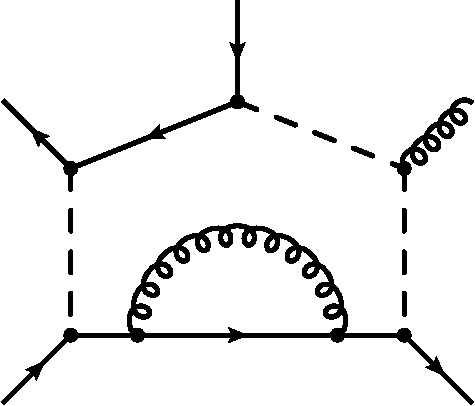
\includegraphics[width=\diagramWidth]{figures/Ds-example-1-1.pdf}}} \quad+\quad
    \vcenter{\hbox{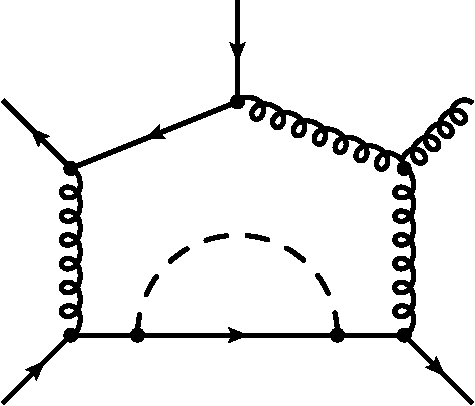
\includegraphics[width=\diagramWidth]{figures/Ds-example-1-2.pdf}}}
    ~\Big) ~\cdot~ (D_s-6) \quad +\\
    &
    \vcenter{\hbox{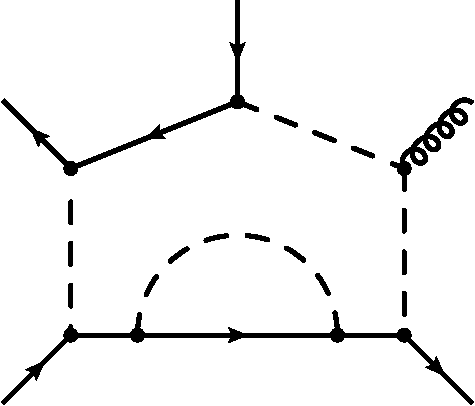
\includegraphics[width=\diagramWidth]{figures/Ds-example-2.pdf}}}
    ~\cdot~ (D_s-6)^2,
  \end{align*}
  \caption{Example of diagrams with scalar particles,
    representing the contributions to the coefficients of $\tilde{\mathcal{K}}_i$ in eq.~\eqref{eq:ds-poly-alt}.
    The thick lines in the diagram on the left-hand side represent particles in arbitrary $D_s$ dimensions.
    The (red) dashed lines connecting external-quark lines represent the traces required to obtain the coefficient of the tensor structure of eq.~\eqref{eq:defAmpsTensb}.
    All particles on the right-hand side are in six dimensions.}
  \label{fig:ds-example-diagram}
\end{figure}


We would like to conclude this section with some remarks.
First, the remaining non-trivial traces of eq.~\eqref{eq:ds-split-traces},
i.e.~those of $\prod_k\gamma^{\mu_k}_{[6]}$, cannot be simplified generically
as the indices appear contracted with the loop momenta at the integrand level.
We evaluate them by the direct summation over a specially constructed set of external states
(in an analogous way to the sums performed in~\cite{Abreu:2018jgq} 
for dimensional reconstruction).
Secondly, in the absence of fermions in the loops, this method coincides with the so called
six-dimensional formalism employed in refs.~\cite{Badger:2013gxa,Badger:2017jhb}, and can 
thus be viewed as an extension thereof to amplitudes with fermions.
Finally, we note that the method presented in this section can be straightforwardly
generalized to higher number of loops by adjusting the base dimension $D_0$,
as well as to the extraction of coefficients of different tensor structures in 
eq.~\eqref{eq:tensorDecomposition}.



\subsection{Unitarity-Compatible Implementation}
decomposition of trees through simplified off-shell recursion.
    Collecting $(D_s-6)$ powers and factors. Implementation in process libraries.

    \todo{Use tree example here}



